\documentclass{beamer}
 
\usepackage[utf8]{inputenc}
\usepackage[english,russian]{babel}
\usepackage{graphicx}
\graphicspath{ {./pictures/} }
\usepackage{color}


\mode<presentation> {\usetheme{default}}
\setbeamertemplate{itemize items}[triangle]
 
\title[Distributed map-reduce]{Курсовой проект \\ \it{Фреймворк и файловая система для распределённой обработки больших данных в рамках концепции map-reduce}}

\author{Выборнов А.И.} % Your name
\institute[МГТУ ИУ-9] {
    МГТУ~им.~Н.~Э.~Баумана \\
    \medskip
    \text{art-vybor@ya.com}
}
\date{\today}

\begin{document}
%----------------------------------------------------------------------------------------
%    Title
%----------------------------------------------------------------------------------------
\begin{frame}
    \titlepage
\end{frame}

%----------------------------------------------------------------------------------------
%   Revierw
%----------------------------------------------------------------------------------------

\begin{frame}
\frametitle{Обзор} 
\tableofcontents 
\end{frame}

%----------------------------------------------------------------------------------------
%   Presentation
%----------------------------------------------------------------------------------------

\section{Постановка задачи}
    \begin{frame}
    \frametitle{Постановка задачи}
        \begin{itemize}
            \item Анализ требований и проектирование архитектуры системы. Реализация нераспределённого map-reduce. Решение проблемы RPC.
            \item Реализация распределённой файловой системы. Реализация фреймворка. Тестирование на примерах.
            
        \end{itemize} 
    \end{frame}

\section{Концепция map-reduce}
    \begin{frame}
    \frametitle{Зачем нужен map-reduce?}
        \begin{itemize}
            \item Обработка больших данных (Big Data).
            \begin{itemize}
                \item Вычисления превосходят возможности одной машины.  
                \item Данные не помещаются в памяти, необходимо обращаться к диску.
                \item Можно хранить много данных, но задержки и пропускная способность оборудования растут пропорционально данным.
            \end{itemize}
            \item Удобная абстракция для построения алгоритмов обработки больших данных.
            \item Устойчивость к отказам.            
        \end{itemize} 
    \end{frame}

    \begin{frame}
    \frametitle{Что такое map-reduce?}
        \begin{itemize}
            \item Структура (key, value) - пара (ключ, значение).
            \item Программирование представляет собой определение двух функций:
            \begin{itemize}
                \item $map: (key, value)\rightarrow[(key, value)]$
                \item $reduce: (key, [value])\rightarrow[(key, value)]$
            \end{itemize}
            \item Между стадиями $map$ и $reduce$ происходит группировка и сортировка данных.
            
        \end{itemize} 
    \end{frame}   

\section{Архитектура}
    % \begin{frame}
    % \frametitle{Архитектура распределённой файловой системы}
    %     \begin{figure}[h!]
    %         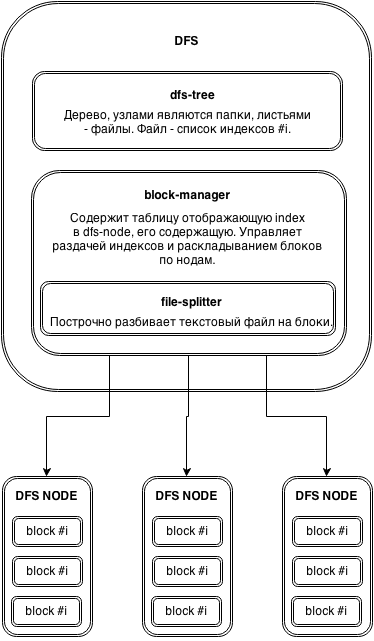
\includegraphics[scale=0.3]{dfs.png}
    %     \end{figure}
    % \end{frame}

    \begin{frame}
    \frametitle{Как работает распределённая файловая система}
        \begin{itemize}
            \item Файл разбивается на блоки фиксированного размера (64мб).
            \item Разбиение файла на блоки порождает генератор.
            \item Получившиеся блоки распределяются по машинам.
        \end{itemize}
    \end{frame}


    % \begin{frame}
    % \frametitle{Архитектура распределённого map-reduce}
    %     \begin{figure}[h!]
    %         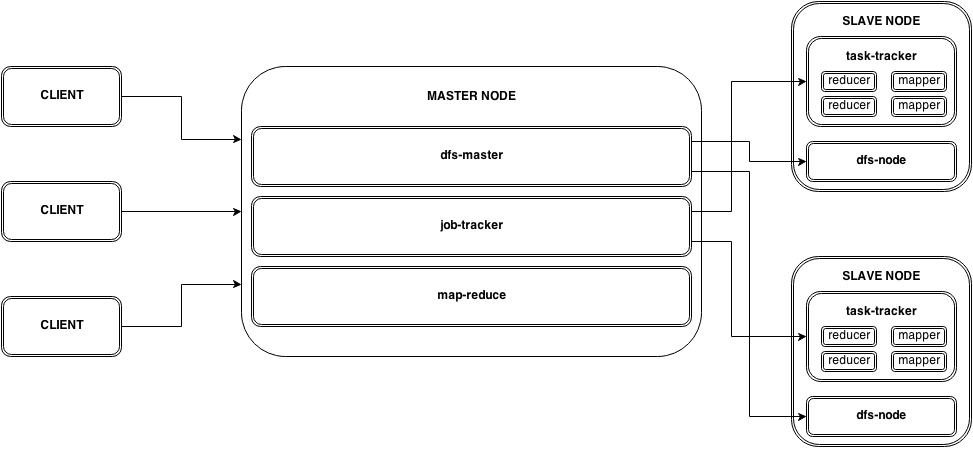
\includegraphics[scale=0.3]{map-reduce.png}
    %     \end{figure}
        
    % \end{frame}


    \begin{frame}
    \frametitle{Как работает распределённый map-reduce}
        \begin{itemize}
            \item На вход получает адреса файлов в DFS для ввода и вывода, а также файл с функциями map и reduce.
            \item Стадии выполнения:
            \begin{itemize}
                \item Получение по входному файлу списка индексов в DFS.
                \item Разбиение списка индексов по узлам.
                \item Выполнение функций map на узлах.
                \item Слияние результатов функций map.
                \item Разбиение полученного результата по узлам.
                \item Выполнение функций reduce на узлах.
                \item Добавление результатов функций reduce в виде файла в DFS.
                \begin{itemize}
                    \item Переименование результатов.
                    \item Запись информации о новом файле в DFS.
                \end{itemize} 
            \end{itemize} 
        \end{itemize}        
    \end{frame}


    \begin{frame}
    \frametitle{Как работает map на узлах}
        \begin{itemize}
            \item По списку индексов получаются данные путём обращения к узлу dfs, находящемуся на этой машине.
            \item Для каждого индекса выполняется переданная функция map.
            \item Результаты всех map аггрегируются в ассоциативный массив (python dictionary).
            \item Полученный результат передаётся на главный узел.
        \end{itemize}        
    \end{frame}

    \begin{frame}
    \frametitle{Как работает reduce на узлах}
        \begin{itemize}
            \item Для каждой полученный пары выполняется переданная функция reduce.
            \item Полученный результат разбивается на блоки равного размера (64мб).
            \item Блоки записываются в dfs на узел, где выполнялся reduce под псевдоименами.
        \end{itemize}        
    \end{frame}


\section{Отчёт}
    \begin{frame}
    \frametitle{Что сделано}
        \begin{itemize}
            \item Разработаны архитектуры распределённых map-reduce и файловой системы.
            \item Реализован распределённый map-reduce.
            \item Для реализации RPC была выбрана связка: ZeroMQ + Marshal.
            \item Реализована распределённая файловая система для хранения больших данных.
        \end{itemize} 
    \end{frame}

    \begin{frame}
    \frametitle{Что предстоит сделать}
        \begin{itemize}
            \item Развить map-reduce для работы с большими данными.
            \item Протестировать полученную систему на больших данных и проанализировать результаты.
        \end{itemize} 
    \end{frame}

\begin{frame}
    \titlepage
\end{frame}

\end{document}